Beide regionalen Klimamodelle wurden mit denselben Daten betrieben: Den Re-Analysedaten und den Simulationsdaten des GCM MPI-ESM-LR 
\section{MPI-ESM-LR} \label{sec:MPI}
Das globale Klimamodell des Max-Planck-Instituts MPI-ESM verbindet Atmosphäre, Ozean und Landoberfläche durch den Austausch von Energie, Momentum, Wasser und $CO_{2}$. Das Modell besteht aus einzelnen Komponenten: ECHAM6 für die Atmosphäre, MPIOM für den Ozean, JSBCACH für die Biosphäre der Landoberfläche und HAMOCC für die Biogeochemie des Ozeans. Für die Verbindung der gekoppelten Komponente HAMOCC und MPIOM zu den restlichen Komponenten über Energie, Momentum, Wasser und $CO_2$ wurde eine eigene Komponente OASIS3 eingeführt. Eine exemplarische Abbildung vom Aufbaus des Modells ist in der Abbildung \ref{fig:mpi-esm} zu sehen. Wegen der derzeitig beschränkten Rechenkapazitäten können komplexe GCMs nur mit einer relativ groben Auflösung von ca 120 -200 km berechnet werden. Für die Vorhersage von Auswirkungen der Klimaänderung benötigt es aber detailliert aufgelöste regionale Komponenten des Klimas. Es gibt mehrere Methoden für das Erhalten der regionalen Daten, wie z.B. RCMs, hoch auflösende GCMs, oder statistische Methoden.
\begin{figure}[h]
	\centering
	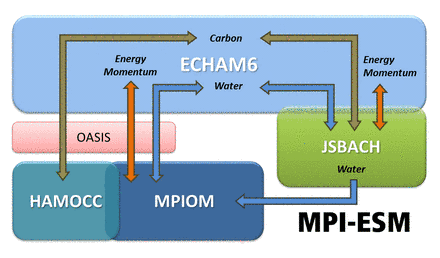
\includegraphics[width=0.7\textwidth]{mpi.png}
	\caption{Aufbau des MPI-ESM, von \cite{mpi-esm-lr}}
	\label{fig:mpi-esm}
\end{figure}
\section{Reanalysedaten}
Reanalysedaten entsprechen dem Abbild des globalen Klimas der Gegenwart oder der nahen Vergangenheit. Diese werden über globale Analysemodelle entwickelt, welche mit einem Zustand der Beobachtungsdaten starten und im Zuge der Simulation stets mit zusätzlichen Beobachtungsdaten gefüttert werden. Ziel dieser Modelle ist es, den physikalischen Annahmen treuen und den Beobachtungsdaten nahen Verlauf zu simulieren, um unter anderem die Güte der physikalischen Annahmen zu evaluieren.
\section{Downscaling-Methoden}
Downscaling hat den Zweck, die Auswirkungen der Daten aus einem globalen Klimamodell, mit einer Auflösung von ca. 120-200km auf regionaler Ebene zu berechnen. Dabei kann entweder eine empirisch statistische Herangehensweise verfolgt werden oder eine dynamisch Modellierte. Durch die empirisch statistischen Methode werden die Beziehungen zwischen der globalen Atmosphären-Konstellation und den regionalen Klimaverhältnissen statistisch quantifiziert. Die größte Herausforderung ist hierbei, geeignete Prädiktoren für den Zusammenhang zu finden. Da es sich bei beiden evaluierten Methoden nicht um Statistische sondern Dynamische handelt, wird nicht näher darauf eingegangen, eine genauere Beschreibung dieser Art von Methode findet man in \cite{RCM}, Kapitel 3. Die dynamische Methode hingegen ist eine
physikalisch basierte, räumliche Interpolation von GCM-Daten. Wie in Kapitel \ref{sec:MPI} erwähnt, gibt es mehrere Downscaling-Methoden:
\begin{enumerate}[label=(\alph*)]
	\item Vereinfachung eines globalen Klimamodells bzw. entkoppeln von sich relativ langsam anpassenden Komponenten z.B. der Ozean-Komponente, die dadurch gewonnene Rechenleistung kann in der höheren Auflösung angewendet werden.
	\item Globale Modelle durch eine variierende räumlichen Auflösung zu vereinfachen. Somit können einige regionale Gebiete höher aufgelöst modelliert werden.
	\item RCM: Die am häufigsten verwendete und in dieser Arbeit auch evaluierte Methode ist, das Einbetten eines räumlich begrenzten Modells in ein globales Modell. Die für das regionale Klimamodell benötigten zeitlich variablen Größen werden dem GCM entnommen und dem Gleichungssystem des RCMs als Randbedingungen zugeführt, somit verfügt das regionale Modelle stets über das aktuelle Abbild der Atmosphäre. Diese Größen müssen nicht zwangsläufig in nur eine Richtung fließen, es kann auch Informationen aus dem RCM zurück in das GCM fließen. Manche hybride RCMs können auch beides, ein und zweifache Flussrichtung der Informationen: von einem in sich selbst gebetteten RCM, fließt Information zum übergeordneten RCM, welches aber abgekapselt in einem GCM gebettet liegt. So kann die Auflösung sukzessive erhöht werden. 
\end{enumerate}
\subsection{Regionale Klimamodelle}
Der zentrale Baustein eines regionalen Klimamodells ist die atmosphärische Komponente, die Austauschvorgänge der Oberfläche werden durch ein interaktiv angekoppeltes Boden-Schnee-Vegetationsmodell erfasst (aus \cite{RCM} Kapitel 4.2f). Für die restliche Bausteine (siehe Abb. \ref{fig:mpi-esm}) werden im einfachsten Fall die vom GCM berechneten Simulationsdaten herangezogen, oder es werden Modelle entwickelt, welche z.B. die regionalen See- und Meeresprozesse nachbilden.\\
Die horizontal Auflösung des Gitters solcher Modelle liegt meist deutlich unter 50km bis zu unter einem km. Aus numerischen Gründen können nur Strukturen (z.B. Gewitterzellen) der vierfachen Gitterweite adäquat berechnet werden. Die vertikale Auflösung beträgt im Normalfall 30-60 Schichten, deren Höhe variiert. Bodennahe Schichten fallen meist dünner als Höhergelegene aus.\\
Im wesentlichen beruhen regionale sowie globale Modelle auf denselben physikalischen Prinzipien: Erhalt der Energie, Masse und des Impulses. Die Gleichungen der Komponenten unterscheiden sich jedoch aufgrund ihrer Formulierungen und besonders in deren Vereinfachungen.
\subsubsection{Atmosphären-Komponente}
Die Atmosphäre besteht im Modell aus dem Gasgemisch feuchte Luft, sowie gegebenenfalls kontinuierlich verteilten Hydrometeoren. Diese sub-Komponenten können dadurch mit einer Dichte, einem Mischungsverhältnisse oder spezifischen Massenanteil beschrieben werden.\\
Für die Beschreibung der gasförmigen Teilchen wird auf die thermodynamische Zustandsgleichung idealer Gase zurückgegriffen.\\
Durch die Hydrometeoren werden Ansammlungen großer Feuchte, wie Wolken Niederschlag beschrieben, wobei die Teilchen der Wolken eine vernachlässigbare Fallgeschwindigkeit und die des Niederschlags eine vereinfacht berechnete Fallgeschwindigkeit aufweisen. Zudem werden die Teilchen noch aufgrund ihres Aggregatzustands (eisförmig, flüssig oder Mischform) unterschiedlich berechnet.\\
Die wichtigsten Zustandsgrößen der Atmosphäre sind die dreidimensionale Geschwindigkeitskomponente, der Druck, die Temperatur, die Dichte und der Partialdruck bzw. Mischungsverhältnisse. Diese Zustandsgrößen beschreiben über Tendenzgleichungen, basierend auf den Erhaltungsgesetzen, den Verlauf der Atmosphäre. Diese Gleichungen sind in RCMs im Gegensatz zu GCMs nichhydrostatisch formuliert. Somit können Abweichungen vom Gleichgewicht der vertikalen Druck- und Gewichtskräfte explizit modelliert werden, was sich in einer hohen vertikalen Dynamik des Modells äußert - dadurch können die Modelle auch auf Auflösungen unter einem Kilometer angewendet werden.\\
An der Atmosphären-Komponente ist wie oben beschrieben die Boden-Schnee-und Vegetationskomponente interaktiv gekoppelt. Diese Komponente beschreibt den Wärme- und Feuchtigkeitstransport der oberen Bodenschichten, den Aufbau und den Abbau von Schneeschichten, sowie den Einfluss der Vegetationsdecke in Bezug auf Energie, Impuls und Masse.
\subsubsection{Parametrisierung} \label{sec:parametrisierung}
Prozesse, die unterhalb der Auflösung des Gitters stattfinden können im allgemeinen nicht vom Modell berechnet werden. Obwohl RCMs relativ hoch aufgelöst sind verbleiben relevante Prozesse nicht abgebildet. Um diese Effekte trotzdem im Modell abbilden zu können wird auf empirisch statistische Verfahren zurückgegriffen. Dazu werden Beziehungen zwischen Beobachtungsdaten und Simulationsdaten errechnet und in den Gleichungen des Modells als skalare Faktoren mit berücksichtigt. Ein Problem dieser skalaren Beziehungen ist, dass davon ausgegangen werden muss, dass die Prozesse sich identisch für zukünftige bzw. vergangene Klimazustände verhalten. Beispiele für diese subskaligen parametrisierten Prozesse sind: molekularer und turbulenter Austausch von Energie, Impuls und Masse (Feuchte), Flüsse an den Grenzschichten zwischen Erdoberfläche und der bodennahen Atmosphäre, Konvektion. Letztere ist problematisch, da Konvektion meistens mit intensiver Wolken- bzw. Niederschlagsbildung verbunden ist. Die Konvektion findet zudem in einer Größenordnung statt, welche ober- und unterhalb der Gitterskala liegt. Somit ist sie besonders schwer in einen subskaligen und einen skaligen Anteil zu teilen. Um dieser Problematik entgegenzuwirken kann die horizontale Auflösung des Modells entweder so verfeinert werden, dass alle konvektiven Prozesse modelliert werden, oder sie so grob zu auszulegen, dass der zu parametrisierende Anteil der Konvektion überwiegt.
\subsubsection{Probleme in der Simulation} \label{sec:problems_in_simulation}
Bei der Simulation eines Modells müssen alle Modellparameter gesetzt werden, dies bedeutet, dass Land-See-Masken, Eisbedeckungs-Masken, Bodentypen einzelner Zellen, und Landnutzungsmasken und eventuell weitere Informationen im Modell spezifiziert werden müssen.\\
Für die Simulation müssen dann noch die zeitabhängigen Parameter wie Luftfeuchte etc. bestimmt werden. Dazu werden die Simulationsdaten eines GCMs oder Reanalysedaten auf die notwendige Auflösung interpoliert. Dadurch können Probleme auftreten da z.B. kleine Inseln erst in einem feinem Gitter abgebildet  werden. Dadurch wird eine Initialisierung der Bodenkomponente für solche Orte notwendig, die im GCM nicht als Landoberfläche abgebildet sind. Zudem werden topographische Einzelheiten wie tiefe Täler im feinen Gitter der RCMs detailgetreuer dargestellt, was eine zusätzliche Höhenkorrektur und Grenzschichtanpassung erfordert.\\
Randbedingungen wie z.B. auf den Bereich des RCMs zulaufende Hoch- und Tiefdruckgebiete werden vom GCM normalerweise alle 3-6 Stunden übergeben, und auf eine zeitlich feinere Auflösung interpoliert. Dadurch können wiederum Probleme auftreten, da die beiden Modelle (GCM und RCM) die Erdoberfläche unterschiedlich darstellen, und sich somit nicht ohne Mehraufwand kompatible Welten ergeben. Dadurch können Wettererscheinungen im Randbereich des RCMs stark zu denen im GCM differieren, da durch die Interpolation nicht alle Daten richtig dargestellt werden. Da es auch keine mathematische Lösungen für die zeitlich abhängigen Zustandsgrößen im genesteten Modell gibt muss können diese nur durch Interpolation berechnet werden. Um solchen Randerscheinungen entgegenzuwirken werden oft einige Gitterzellen am Rand als Pufferzone eingesetzt, in welchen die internen Lösungen mit den extern zugeführten Daten kombiniert werden und dem Abstand zum Rand entsprechend gewichtet werden. Dieser Lösungsansatz wird oft auch mit ''Nudging'' kombiniert, wo Wetterinformationen nicht nur am Rand sondern auch innerhalb des Bereichs ausgetauscht und verglichen werden (vgl. \cite{RCM} Kapitel 4) Bei den evaluierten Datensätzen ist besonders in Kapitel \ref{subsec:eval_alp3} ein solches Phänomen zu beobachten, wo am Rande des Modellbereichs extreme Differenzen zu den Beobachtungsdaten herrschen.
\subsection{CCLM4-8-17}
CCLM ist die Klimaversion (CLM) des Wettervorhersage-Modells COSMO, entwickelt vom Potsdamer Institut für Klimafolgenforschung, dem Helmholtz-Zentrum Geesthacht, und der BTU Cottbus, basierend auf dem Lokalmodell des Deutschen Wetterdienstes. Die Grundversion besteht aus einer nicht-hydrostatischen Atmosphären-Komponente und einer angekoppelten Boden-Vegetationskomponente.\\
CCLM4-8-17 ist ein regionales Klimamodell, in welchem die Konvektion wie zuvor beschrieben parametrisiert dargestellt ist. Hier scheinen sich die Probleme der Randbedingungen nicht so stark abzuzeichnen wie im CCLM5-0-9 (siehe Kapitel \ref{chap:quantile_seasons}). Die Auflösung dieses RCMs beträgt ungefähr 12.5km und musste auf die Auflösung der Beobachtungsdaten interpoliert werden, was auch zu leichten Fehldarstellungen führen kann, da sich die Werte der einzelnen Gitterzellen unterscheiden können (siehe Kapitel \ref{chap:intro}). Jedoch waren die Ergebnisse für dieses Modell relativ gut (siehe Kapitel \ref{chap:conclusion}). Nur die Schwankungen des Starkregens sind nicht adäquat dargestellt, was auf die Parametrisierung zurückzuführen ist (siehe Kapitel \ref{chap:quantile_seasons}),
\subsection{CCLM5-0-9}
\begin{wrapfigure}{r}{0.5\linewidth}
	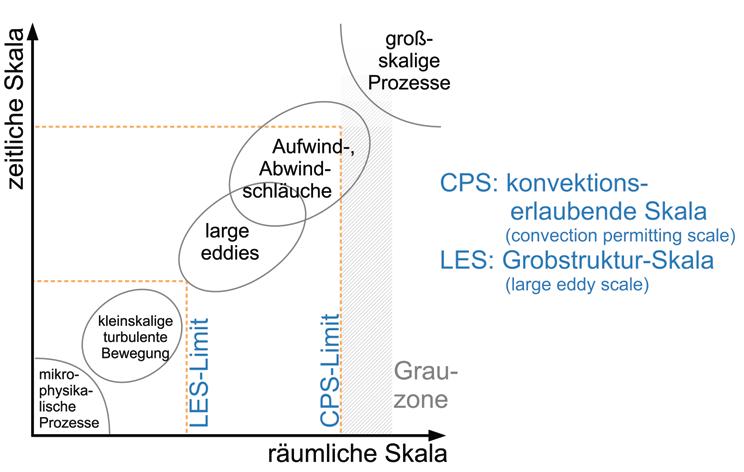
\includegraphics[width=0.49\textwidth]{konvektion.png}
	\caption{Raumzeitliche Skalen der Konvektion, Bild aus \cite{RCM}. Large eddies bezeichnen die kleinsten nicht vernachlässigbaren turbulente Wirbel auf einer Gitterweite von 10-100m. CCLM5-0-9 liegt durch eine Gitterweite von 3km innerhalb des CPS-Limits, aber außerhalb des LES-Limits.}
	\label{fig:konektion-skala}
\end{wrapfigure}
Dieses RCM hat eine weitaus feinere Auflösung von 3km bzw. $0.1 ^\circ$, somit kann, wie in Kapitel \ref{sec:parametrisierung} beschrieben, die Konvektion explizit simuliert werden. Wie im Artikel \cite{convective_phenomena} angemerkt ist, hat dies den Vorteil, dass die Konvektion auf physikalischen Gesetzen basiert. Dadurch kann sie auch für ein global verändertes Klima wissenschaftlich fundierte Aussagen liefern. Da so die Konvektion nicht statistisch abhängig vom derzeitigen Klimazustand gemacht wird.\\
Die Konvektion ist auch in diesem Modell teilweise parametrisiert (vgl. Abb. \ref{fig:konektion-skala}, dies betrifft Phänomene die unterhalb der Gitterweite ablaufen wie z.B. die trockene flache Konvektion. Es wird also angenommen, dass atmosphärische Turbulenzen nicht auf dem Gitter repräsentiert und somit parametrisiert werden (vgl. \cite{RCM} Kapitel 4). Die Parametrisierung erfolgt über thermodynamische Gesetze und Umwandlungsraten. Es wäre auch nicht sinnvoll, die Konvektion vollends zu modellieren, da dazu eine Gitterweite von ca. 0.1mm notwendig wäre. Die large eddies (siehe Abb. \ref{fig:konektion-skala}) bezeichnen die kleinsten nicht vernachlässigbaren konvektiven Prozesse, und sind mit einer Gitterweite von ca 50m abbildbar. Der rechnerische Mehraufwand bringt aber nicht unbedingt einen Mehrwert in den Ergebnissen, wie Byran et al. in \cite{bryan} zeigten. Durch eine Gitterweite von ca 4km sind die konvektiven Prozesse in Wolken hinreichend abbildbar.
Das Modell basiert auf der neueren Version des COSMO - Modells. Jedoch sollte angemerkt werden, dass die Konvektions-Komponente noch nicht sehr lange existiert, somit konnte sie bisher noch nicht hinreichend getuned werden.
Die Daten (ALP-3) die in dieser Arbeit untersucht werden kamen durch ein nesting in das RCM CCLM4-8-17 zustande.
